\section{Simulation Results}
%======================================================================================
% Include the plot of the robot's trajectory through the maze.

The robots trajectory through the maze can be seen in Fig.\:\ref{fig:robot_path}. The lines appear to be perfectly straight, however they are not. The deviation is a function of the number of decimals used in the approximate position of obstacles, with the deviation from the straight line increasing as the number of decimals decrease, and the trajectory becoming more parabolic. No exact relationship or function was established for this relationship.
\begin{figure}
    \centering
    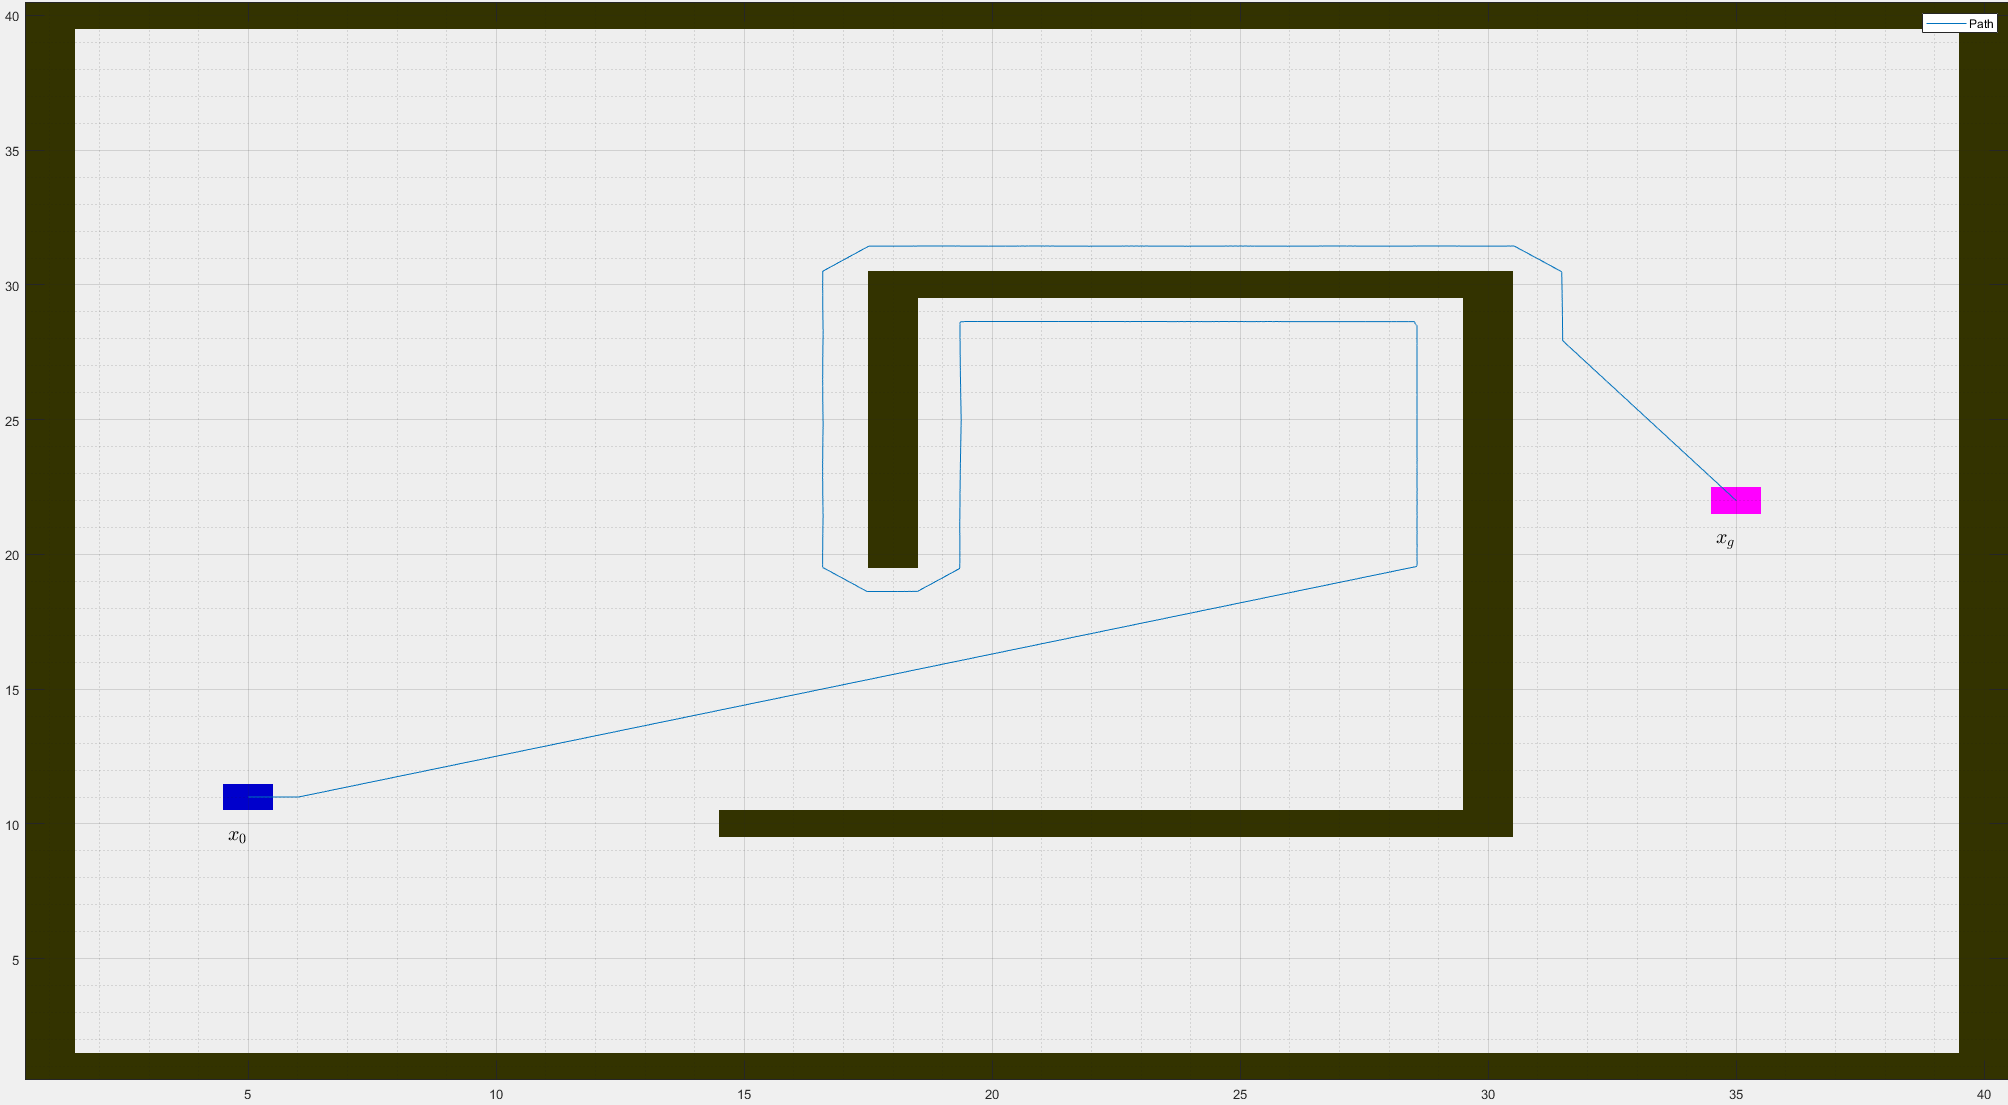
\includegraphics[width=\columnwidth]{images/robot_path.png}
    \caption{Trajectory of the robot through the maze.}
    \label{fig:robot_path}
\end{figure}

%======================================================================================
% Present three subplots

The subplot shown in Fig.\:\ref{fig:x_time} shows x of the robot as a function of time. In subplot Fig.\:\ref{fig:y_time} the same is shown but for y. $\theta_{\text{ref}}$ compared to $\theta$ with respect to time is shown in Fig.\:\ref{fig:theta_time}. The heavy clipping occuring in Fig.\:\ref{fig:theta_time} is the result of constraining all angles to $[-\pi, \pi]$, therefor angles close to $-\pi$ or $\pi$ can jump between the two when incremented or decremented slightly.
\begin{figure}
	\centering
    \begin{subfigure}[t]{0.32\columnwidth}
		\centering
		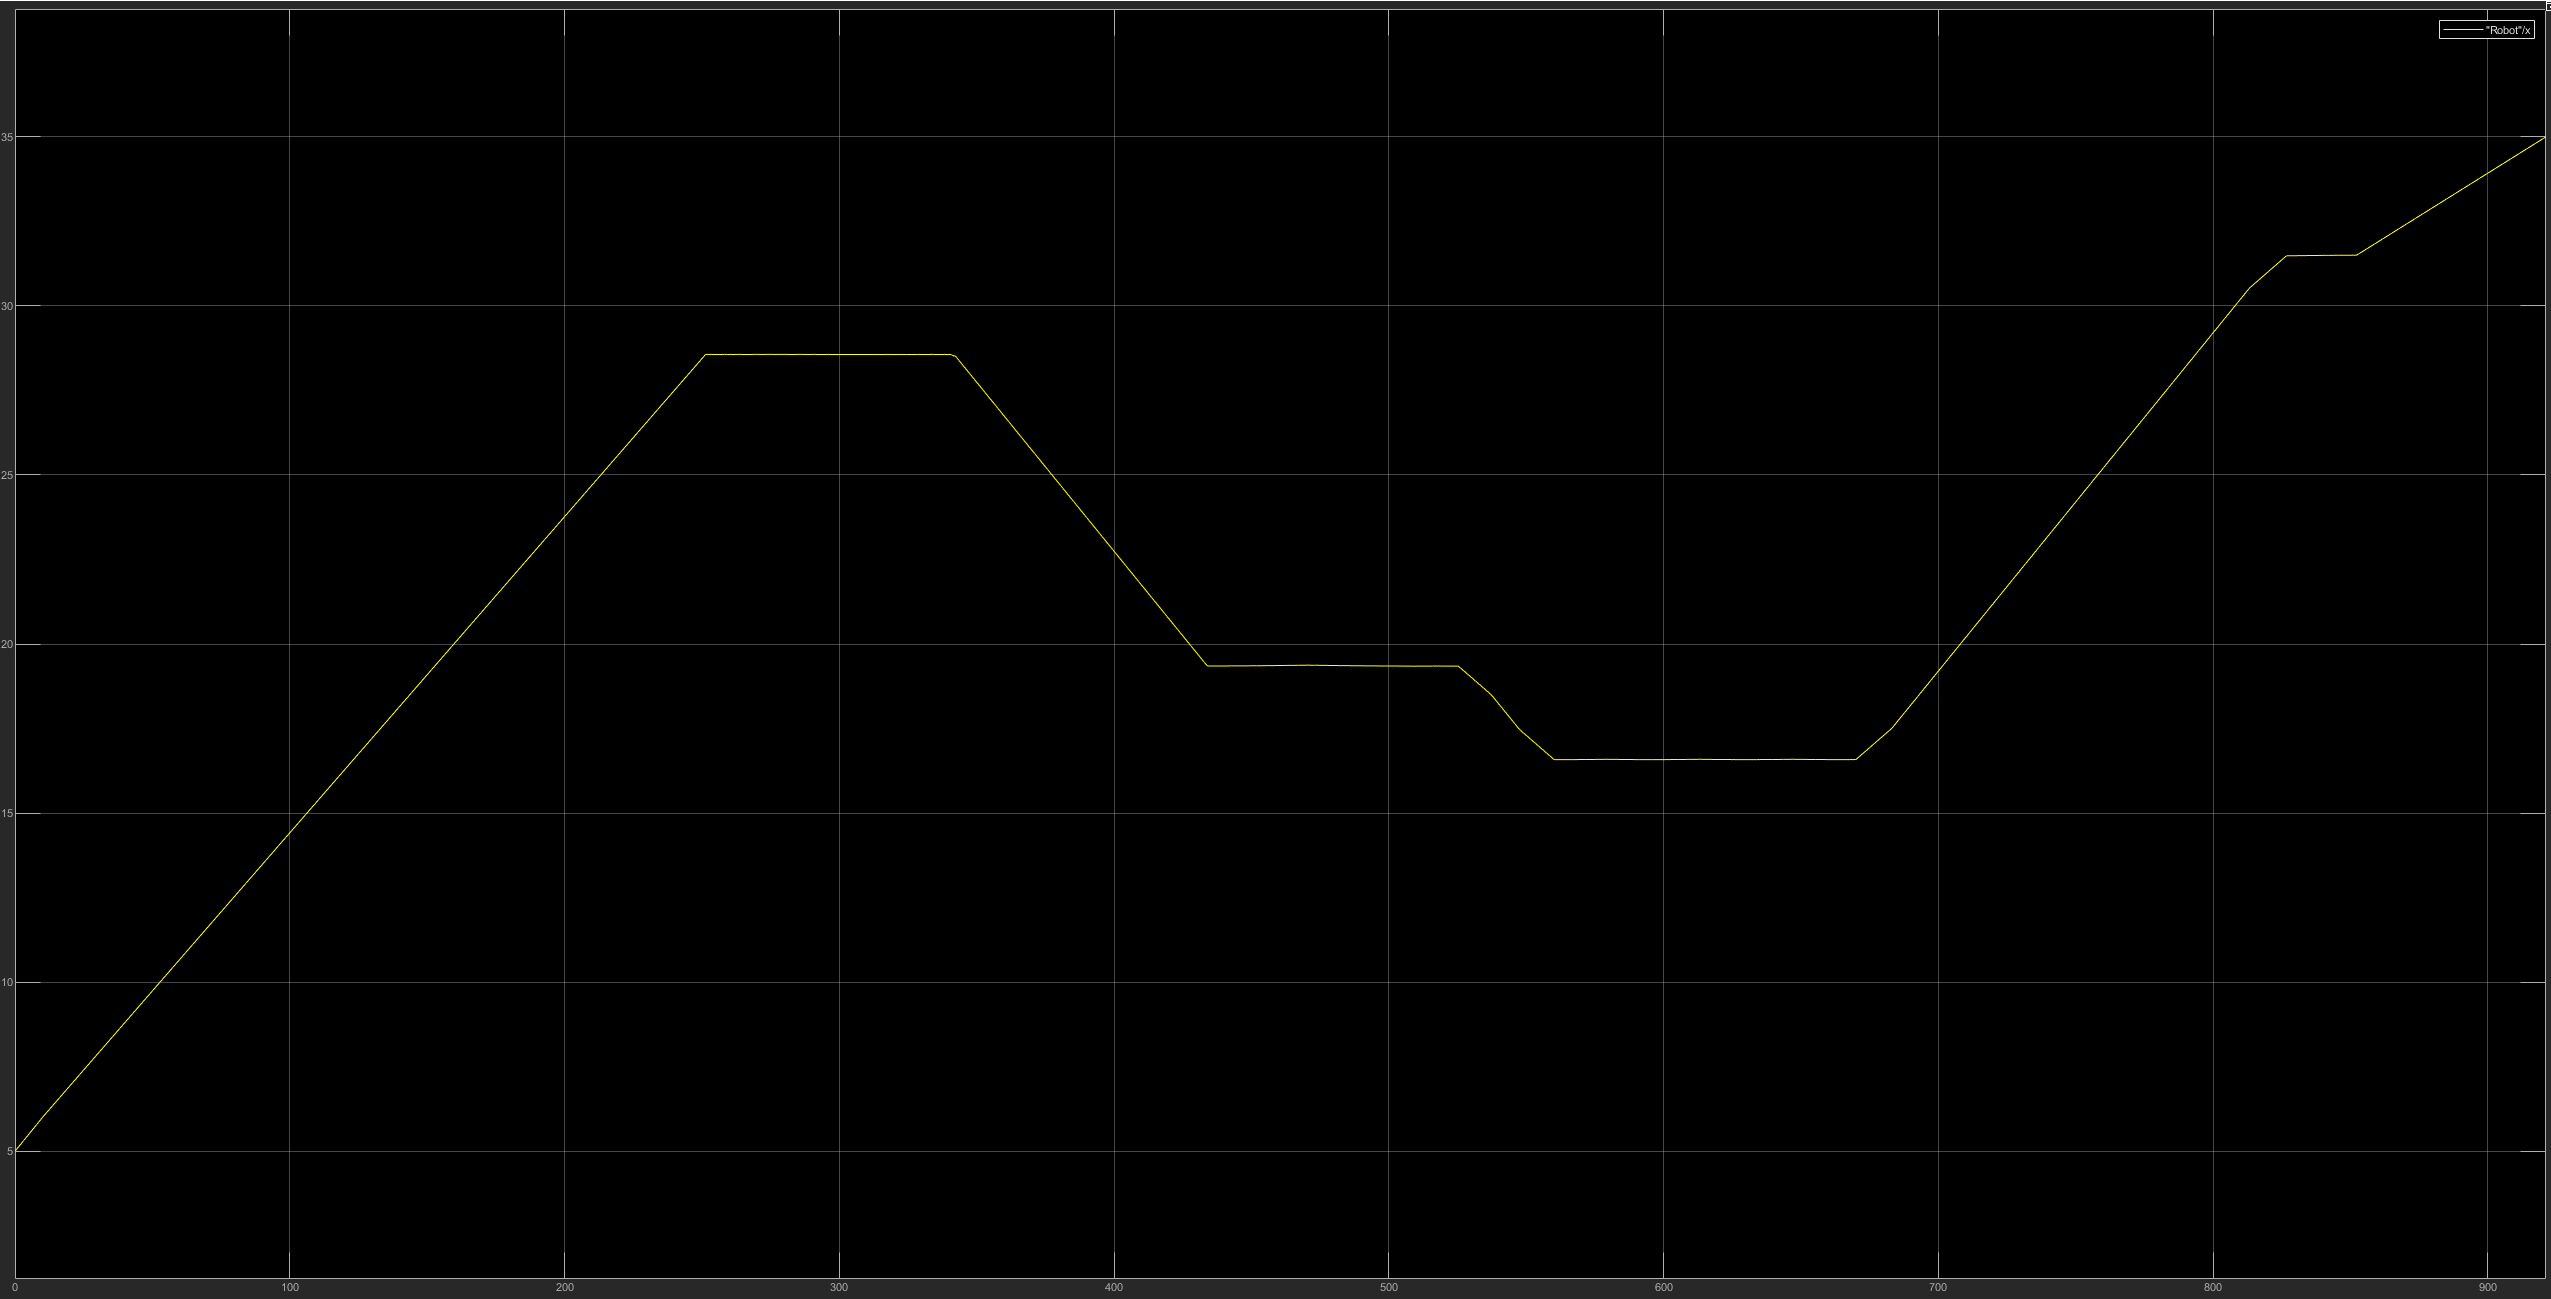
\includegraphics[width=\textwidth]{images/x_time.png}
		\caption{x coordinate of the robot as a function of time.}
        \label{fig:x_time}
	\end{subfigure}
    \hfill
	\begin{subfigure}[t]{0.32\columnwidth}
		\centering
		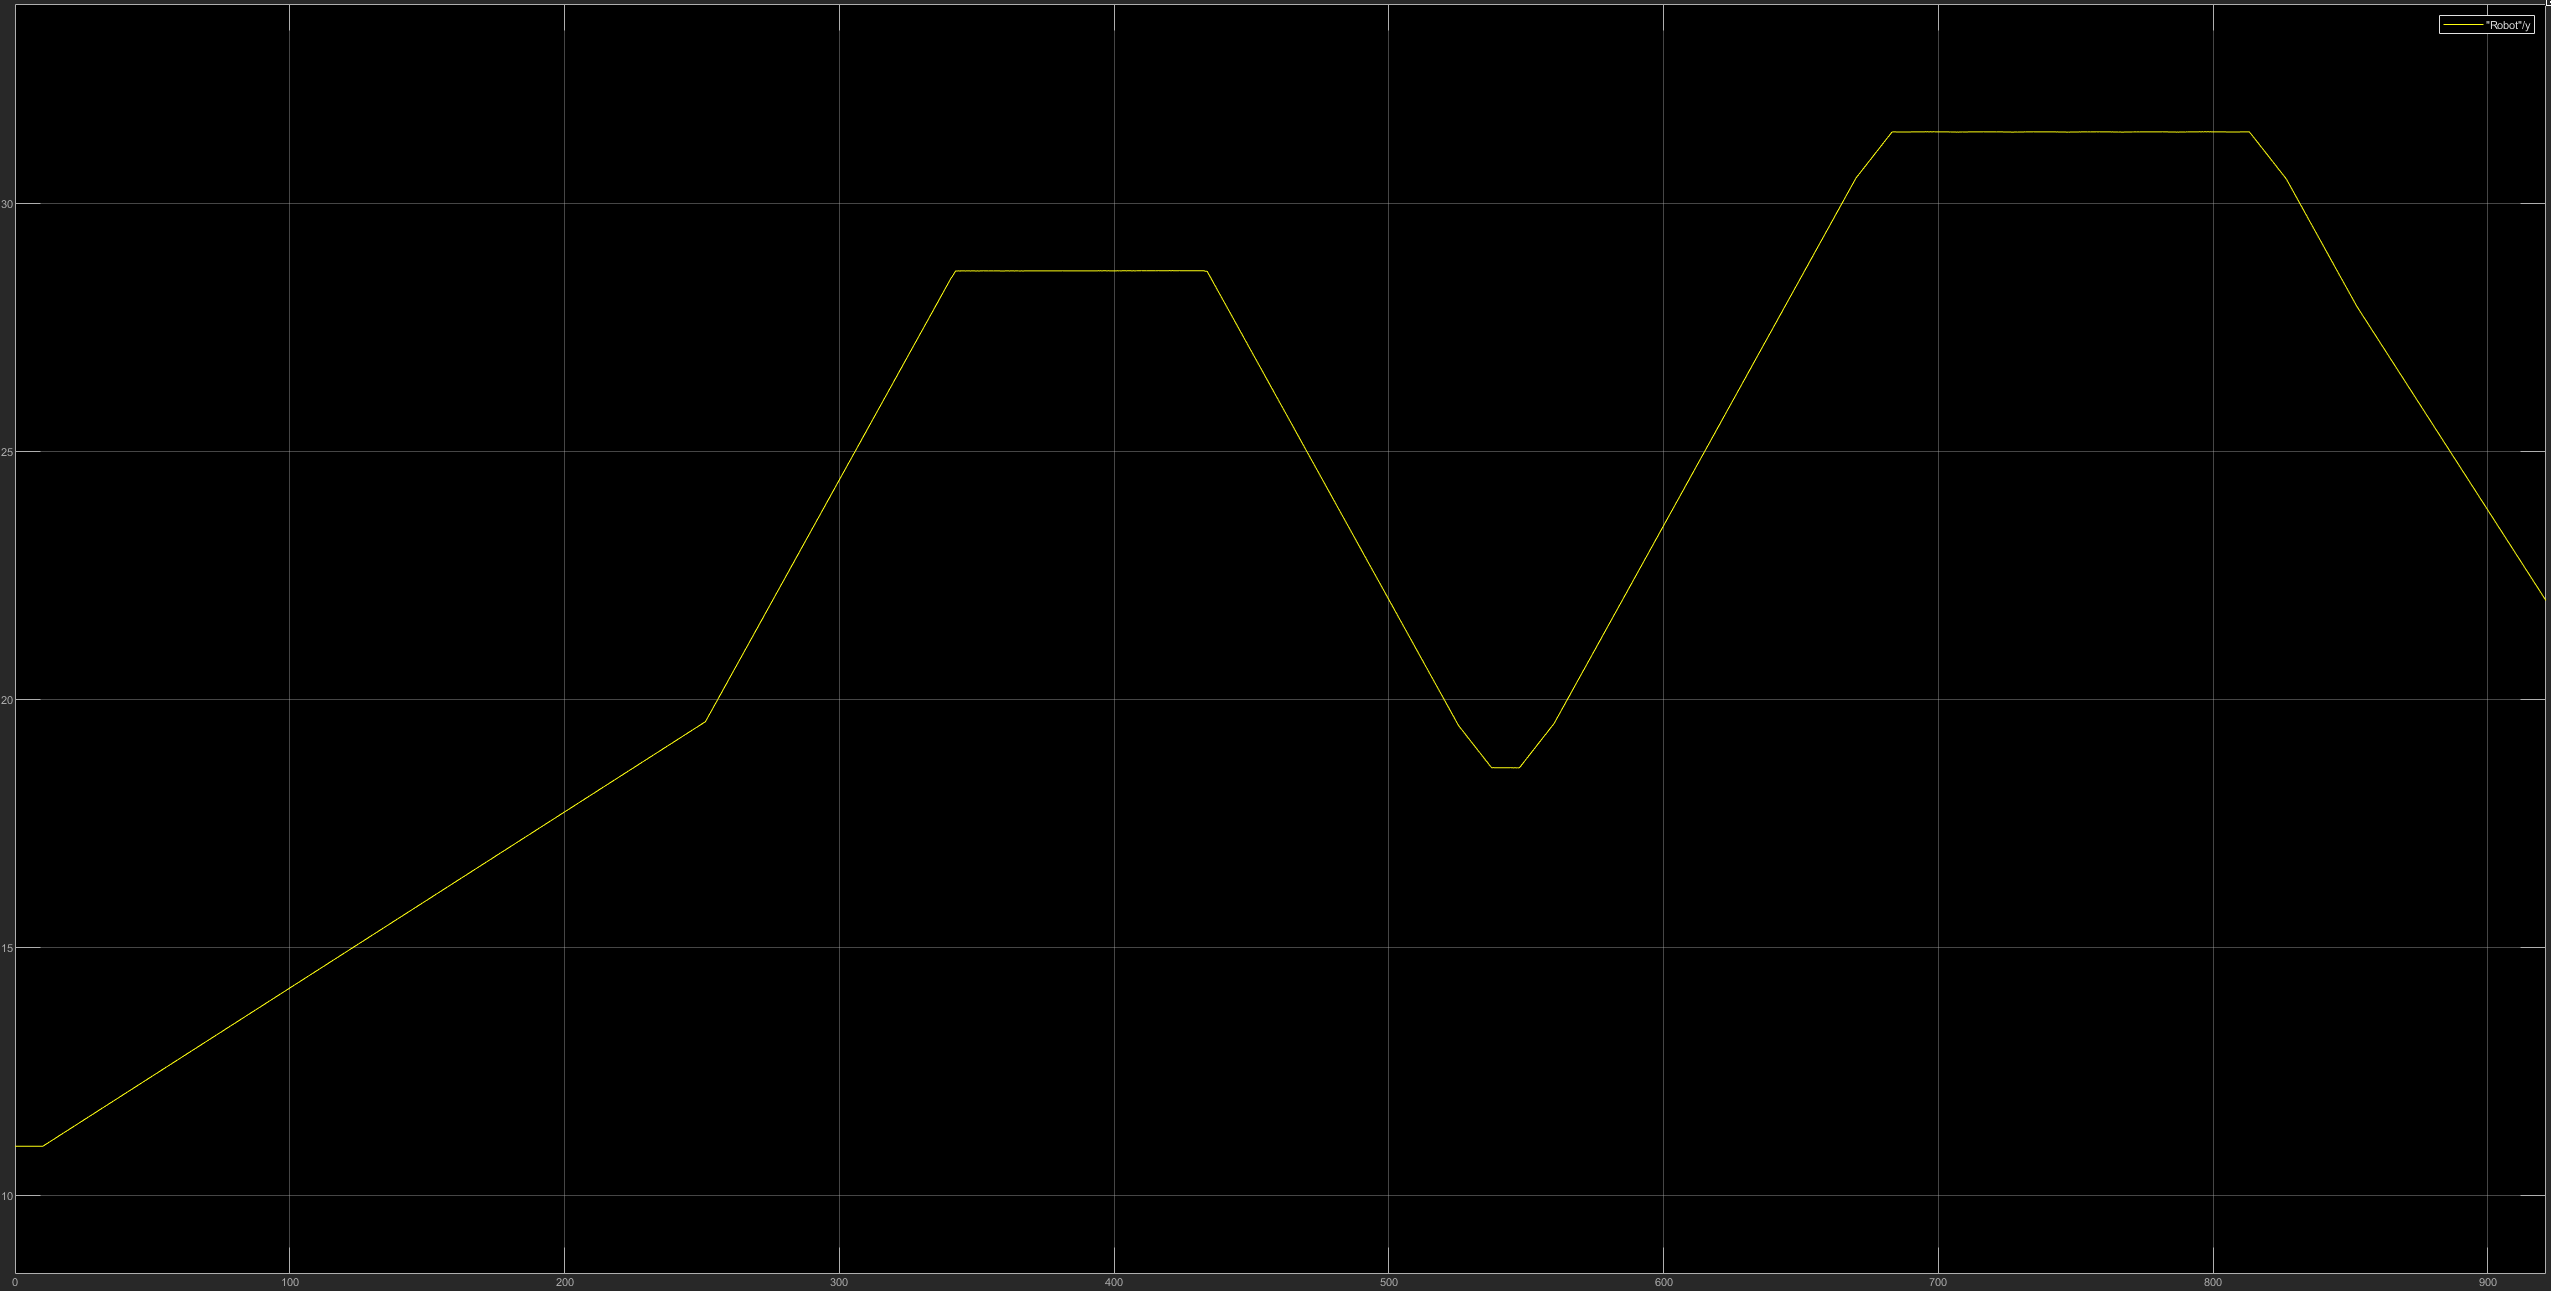
\includegraphics[width=\textwidth]{images/y_time.png}
		\caption{y coordinate of the robot as a function of time.}
        \label{fig:y_time}
	\end{subfigure}
    \hfill
    \begin{subfigure}[t]{0.32\columnwidth}
		\centering
		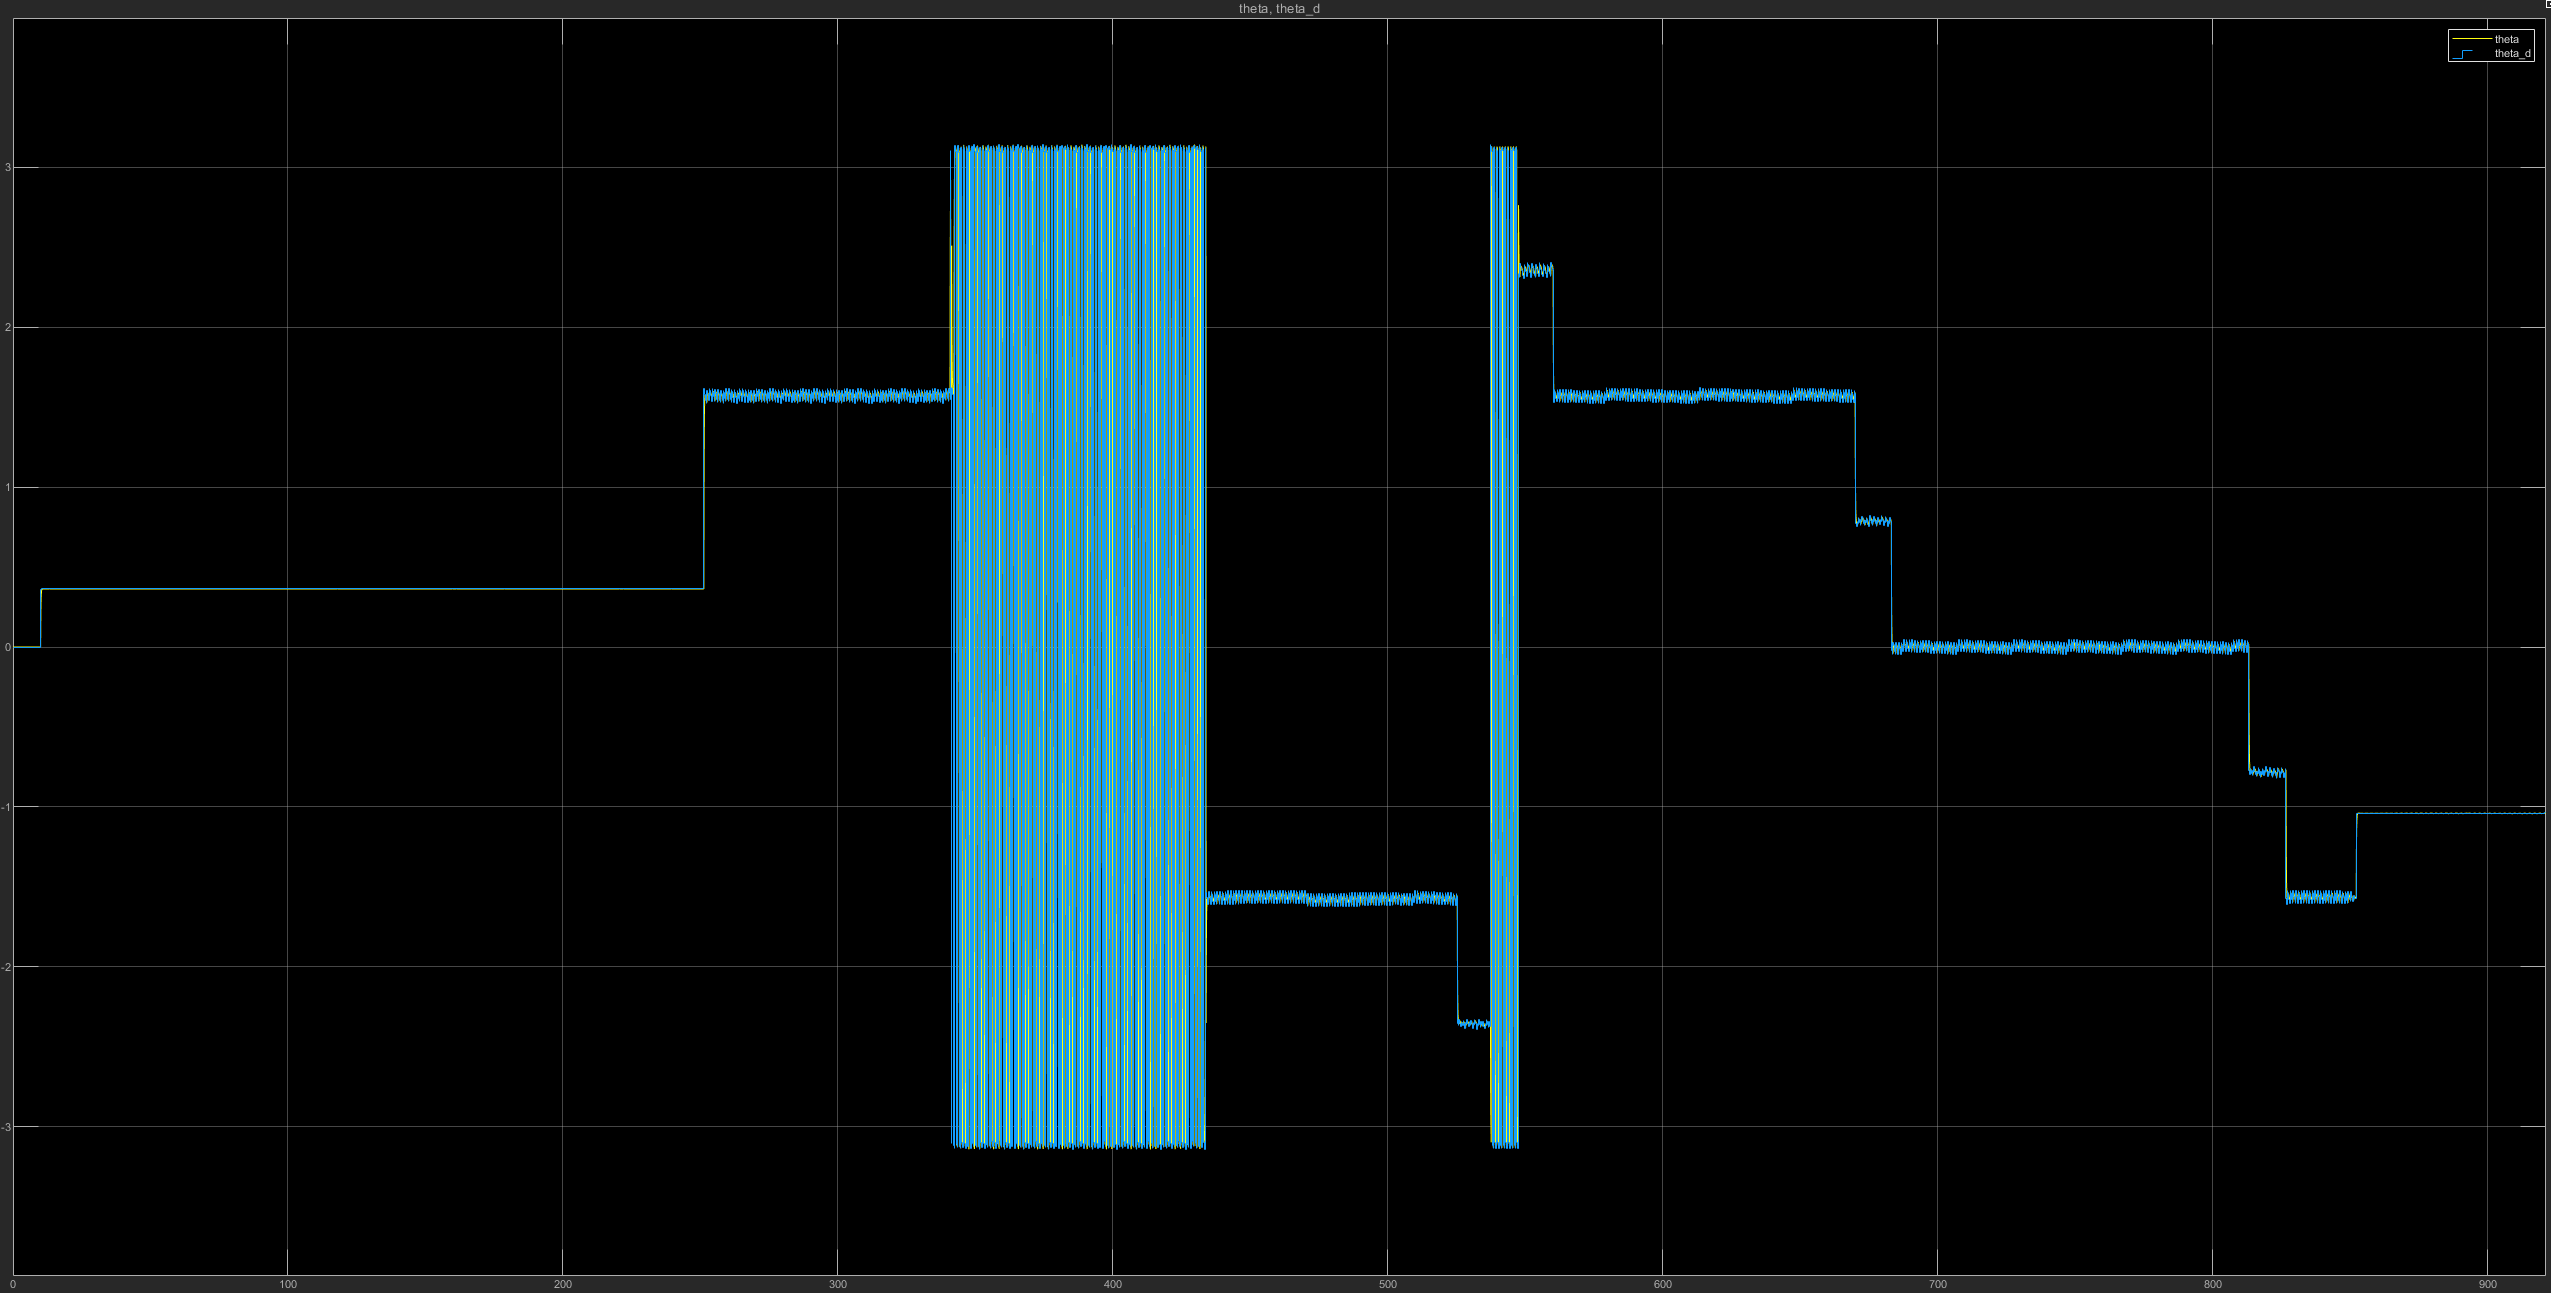
\includegraphics[width=\textwidth]{images/theta_time.png}
		\caption{$\theta_{\text{ref}}$ ($\theta_{\text{desired}}$) compared to $\theta$ of the robot as a function of time.}
        \label{fig:theta_time}
	\end{subfigure}
	\caption{Robot pose as functions of time.}
    \label{fig:x_y_theta_sub}
\end{figure}

%======================================================================================


%======================================================================================
\begin{comment}
    
\end{comment}
%======================================================================================